\section{The model and the task}
\label{sec:model}

This section defines the smallest system that shows the process we care about, the one parameter that controls it, and the quantity a simulator has to produce. We need a process in which a cluster switches between two arrangements by tunneling, a timescale for that switch, and an observable that records it; every cost in later sections is the cost of producing that observable up to that time.

\begin{figure}[t]
\centering
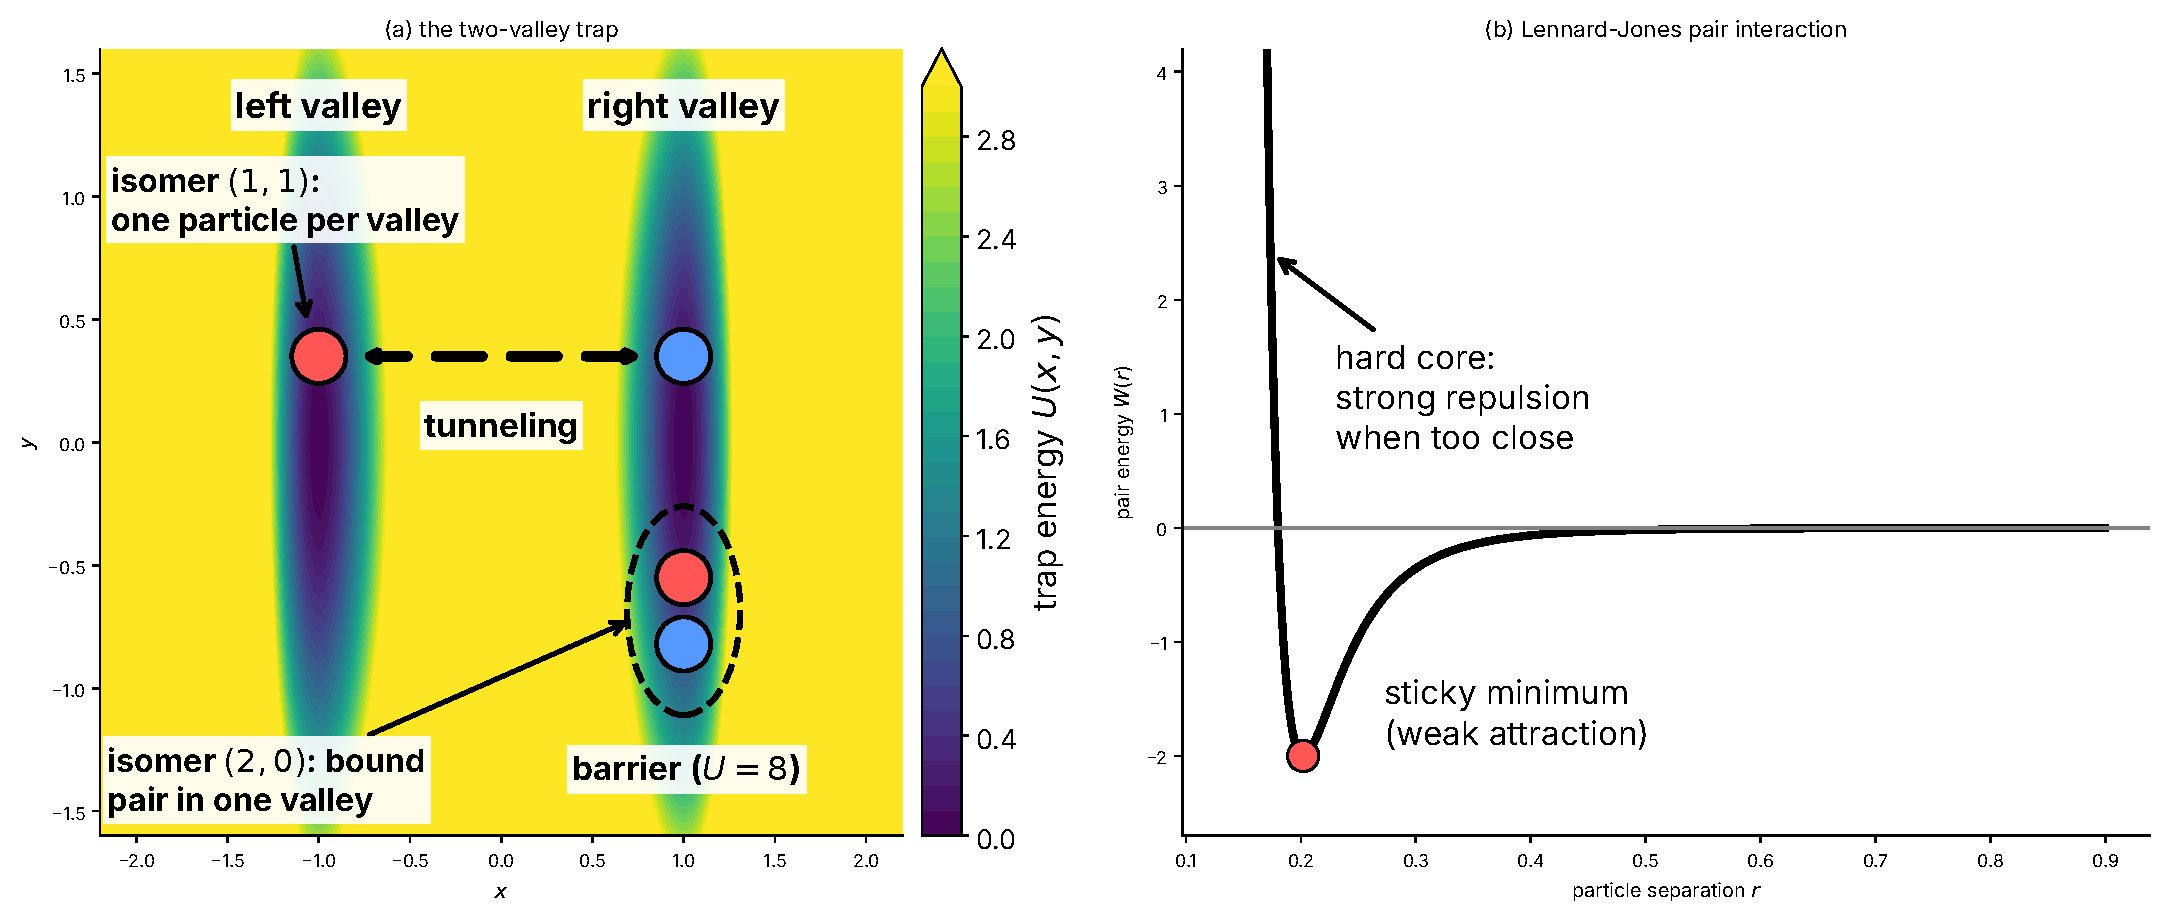
\includegraphics[width=0.95\textwidth]{figures/fig_model.pdf}
\caption{\textbf{The model.} (a) The two-valley trap (colour scale clipped at $U=3$, so the barrier, of height $U=A=8$,
appears uniformly bright), the two isomers of a two-particle cluster and the tunneling path between them.
(b) The capped Lennard-Jones pair interaction: hard core at short range, a shallow minimum at $r_{\min}$.
Parameters: Table~\ref{tab:params}.}
\label{fig:model}
\end{figure}

\paragraph{System.}
Each particle moves in two dimensions in a trap with two valleys, $U(x,y)=A(x^2-1)^2+\tfrac12\omega_y^2y^2$ (Fig.~\ref{fig:model}a): the valleys lie at $x=\pm1$ and are separated
by a hill of height $A$ that a particle cannot climb but can tunnel through. A tilt $c\,x$ added to each particle makes one valley deeper. Two particles at
distance $r$ repel at short range and attract weakly at long range through the Lennard-Jones potential $W(r)=4\epsilon[(\sigma/r)^{12}-(\sigma/r)^{6}]$, capped at $V_{\rm cap}$
(Fig.~\ref{fig:model}b). The interaction range is small compared with the valley separation, so particles interact only
when they share a valley, and the cluster is described by \emph{how many particles sit in which valley}: the occupation isomers,
$(1,1)\leftrightarrow(2,0)$ for two particles, $(N-1,1)\leftrightarrow(N,0)$ in general. The Hamiltonian is the sum of the kinetic energy, the trap, the tilt and the pair interactions,
\begin{equation}
\hat H_N(c)=\sum_{i=1}^{N}\Big[-\tfrac12\nabla_i^{2}+U(x_i,y_i)+(c+c_i)\,x_i\Big]+\sum_{i<j}W(|\mathbf r_i-\mathbf r_j|),
\qquad c_i=(i-1)C_0 .
\label{eq:HN}
\end{equation}
The tilt is tuned to the \emph{resonant} value $c^*(N)$ at which the two isomers have the same energy; they then mix completely and tunneling between them is fastest. The small offsets $c_i$ make
the particles non-identical (labelled, like different isotopes), which is the harder case for classical methods. The observable is the number of particles in the right valley,
\begin{equation}
\hat O=\sum_{i=1}^{N}\Theta(x_i),\qquad \|\hat O\|=N .
\label{eq:Oobs}
\end{equation}
It changes by one when one particle crosses the barrier, so it is the direct readout of the isomer switch. On the grid one column lies exactly on the barrier top; it counts with weight $\Theta(0)=\tfrac12$, so the two valleys are treated alike (Appendix~\ref{app:numerics}).

\paragraph{The one knob.}
Rescaling lengths by $\sigma$ and energies by $\epsilon$ leaves one dimensionless mass, $\muq=m\sigma^2\epsilon/\hbar^2$. What matters for tunneling is not the mass itself but how heavily it weighs on the barrier: the \emph{action under the barrier}
$S_0=\tfrac43\sqrt{2mA}\,a/\hbar$ ($a=1$ the half-separation of the valleys), and the tunneling time grows as $e^{S_0}$~\cite{helffer1984,garg2000}. We therefore use the \emph{trap-units} mass $\mut:=\tfrac32S_0$, for which the tunneling time grows as $e^{2\mut/3}$.
The simulations run at one light point, $\mut=\num{mut0}$
($S_0=\num{Szero}$, $\muq=\num{muzero}$), where one isomer transfer takes $t_0=\num{tstar0}$ (the two-particle switching time $\pi/\dE_2$ measured on the position grid; Appendix~\ref{app:numerics}). In an optical lattice of depth $s$ recoil energies the barrier action is $S_0=2\sqrt s$ for every
species, so $\mut=3\sqrt s$ and the mass drops out of the single-particle part of the tunneling time (Appendix~\ref{app:proofs}); this is
a statement about the single-particle action only, since the pair-interaction cost of Appendix~\ref{app:quantum} differs between species.

\paragraph{The task.}
In words: start the cluster in one arrangement, let it evolve, and report how many particles are in the right valley as a function of time, with a stated accuracy, until the first full transfer. A simulator that can do this has reproduced the tunneling.
\begin{defn}[Task]\label{def:task}
Given a valley-localized start $\psi_0$, approximate $f(t)=\langle\psi_0|e^{i\hat H_Nt}\Op\,e^{-i\hat H_Nt}|\psi_0\rangle$ for $0\le t\le\Tobs$ to additive error
$\varepsilon\|\Op\|$.
\end{defn}
For a clean doublet (two levels well separated from all others) of splitting $\dE_N$ the observation time is the first isomer transfer, $\Tobs=\pi/\dE_N$; where no clean doublet exists we use the
first minimum of $\langle\Op\rangle(t)$. The cost of a quantum simulation grows with $\Tobs$, so we need $\Tobs$ at masses other than the simulated one. With the semiclassical dependence on the barrier action, anchored to the measured two-particle value,
\begin{equation}
\Tobs(N,\mut)=g_N\,t_0\,e^{2(\mut-\mut_0)/3}\Big(\frac{\mut_0}{\mut}\Big)^{1/2},\qquad g_N=\frac{\dE_2}{\dE_N}.
\label{eq:Tobs}
\end{equation}
The factor $g_N$ says how much slower the $N$-particle transfer is than the two-particle one. Equation~\eqref{eq:Tobs} is an interpolation anchored to a measurement, not an ab-initio law; at $S_0=\num{Szero}$ the asymptotic regime is not reached. The gap ratio $g_N$ enters the quantum
price linearly (a ratio $g_N>1$ lowers the quantum edge by $\tfrac32\ln g_N$). We carry $g_N=1$ and test it where a clean doublet exists
(Appendix~\ref{app:numerics}).

\paragraph{Representations and starts.}
The same $\hat H_N$ can be written in three ways, and each route of Section~\ref{sec:framework} needs a different one (Table~\ref{tab:params}). \emph{Basis 1}, the position grid, has $d=M=\num{M_grid}$ cells per particle and $d^N$ amplitudes; the exact-storage count and the cost models refer to it. \emph{Basis 2}, the mode basis, keeps the lowest $k$ eigenstates of each particle's own one-particle Hamiltonian
($d=k$); all entanglement measurements use it, because the grid state does not fit in memory beyond $N=3$. Its price is truncation of the correlation hole between particles
that share a valley, so every mode-basis entropy is quoted with its spread over $k$. \emph{Basis 3}, the qubit register, is the grid written in binary,
$n_p=\lceil\log_2M\rceil=\num{n_p}$ qubits per particle; it is used only to count quantum cost, and no quantum computation is simulated.
Two starts are used. The \emph{product start} is a product of one-particle valley orbitals; it ignores the correlation hole between particles in the same valley, which
makes it a quench for $N\ge3$. The \emph{correlated start} is the ground state of $\hat H_N+W\sum_iP^{\rm wrong}_i$ with a penalty of strength $W$ (not the pair energy $W(r)$) on the wrong side for each particle; it
contains the pair correlation and is the physically relevant isomer. Preparing it on a quantum computer costs extra, which the quantum price of Section~\ref{sec:quantum} does not include.
All entropy results below are for the correlated start unless stated.
